\chapter{Detecting crucial parts of the input Simplifying Inputs} \todo{better title}
\label{cha:3}
When we detect that the PUT crashes, wrongly satisfies, wrongly not satisfies or hangs on a given input we now want to know why it does that. What causes this unwanted output and what line the bug occurs. With crashes, a stack trace and some luck this could be easy, but when the crash is not main perpetrator or we get an other unwanted output the developer my need to debug deep into the code to find the bug. This with a potential large input could be a tedious and long assignment, for this reason we would like to know what parts of the input are related to the bug. We will discover this further in this chapter, starting with \todo{plug in sections}

\section{Deobfuscating inputs}
When receiving a big input the chance of having parts unrelated to the bug is almost guaranteed, we will call them (unintentionally) obfuscated inputs. Deobfuscating those takes a lot of try and error to see if the bug is still there\cite{bookZellerwhyProgramsFail} or having to walk through the execution to find the bug. With deobfuscating inputs we not only help the developer to find the bug faster, we can also group similar bugs and deduplicate error reports (more on that later). 
\section{The precision effect}
With one caveat to take in mind we need to be careful to still find the same bug and to not change a null pointer dereference bug to a parser related bug. This, as discussed in the previous chapter, is due to some bugs being more important than others. In a paper by Andreas Zeller and Ralf Hildebrandt \cite{5zeller2002simplifyingIsolatingFailure-inducing} talk about this exact problem which they called "the Precision Effect". sometimes this is not a problem, for example when we are trying to find all possible bugs and will rerun the fuzzer after each incremental improvement or when a deeper bug turns into another deep bug.

 Finding these crucial parts of inputs is where the following techniques come into play.
\subsection{Simplifying}
The first technique is the simplification of inputs, where we remove parts of a failing input and check if it still fails and often called "delta-debugging"\cite{bookZellerwhyProgramsFail}. When it is no longer possible to remove any part of the input we have obtained an input where all parts are needed to expose the bug. This input is at the same time also the shortest possible input to trigger this bug, making finding the bug easier than in the original input filled with unrelated parts.
\subsection{Isolation}
Another technique, isolation, is explained by Andreas Zeller et al. 
\cite{5zeller2002simplifyingIsolatingFailure-inducing} this is a technique where instead of minimizing the input we try to find the smallest difference between an input that shows the bug versus an input that does not show the bug. This with the advantage that no matter if we find the bug or not the difference will diminish, either the maximum input will shrink or the minimum input will grow. This technique brings extra complexity with the tracking of multiple inputs and the maximal input could take longer to run due to its size, but according to Andreas Zeller et al. this is the faster one to the two. Figure
\ref{fig:simplificationIsolation} shows the difference between simplifying and isolation, both finding the critical part of the input, with simplification the critical part is indicated by the last test in the figure while with isolation it it the differenc of the passed and failed test.
\begin{figure}
	\centering
	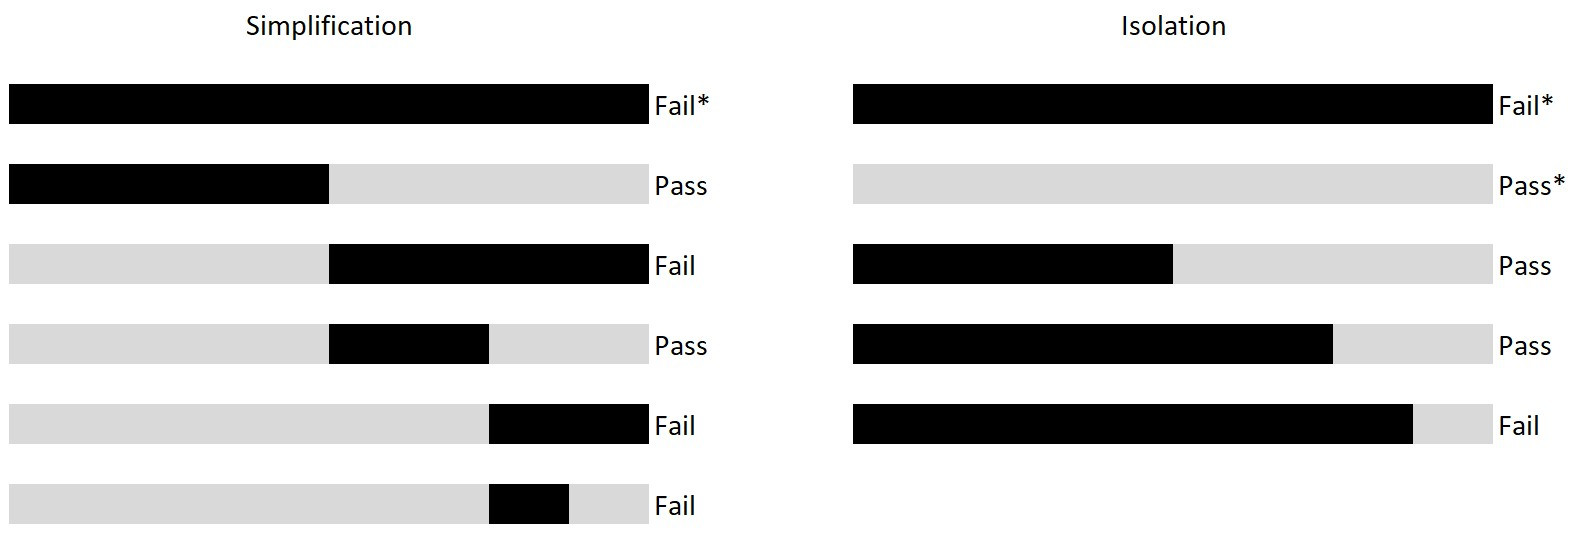
\includegraphics[width=1.0\textwidth]{images/simplificationIsolation}
	\caption{Deobfuscating inputs based on simplification (left) and isolation (right) on the same input. The '*' indicates that the result is already known and does not need to be recalculated. Figure based on an illustrations found in\cite{bookZellerwhyProgramsFail}.}
	\label{fig:simplificationIsolation}
\end{figure}

\subsection{Small inputs by creation}
An interesting approach by Alexandra Bugariu and Peter M\"uller\cite{9bugariu2020automaticallyTestingStringSolvers} is to forgo the need of deobfuscating inputs by generating inputs "small by construction".

\section{What size to change}
Something we glossed over so far this chapter is the chuck sizes to remove while trying to find the critical parts of the inputs. The previous seen techniques will work well on the original fuzz testing Miller et aL.\cite{4originalFuzzingUnixUtils} worked on since those random generated symbols where independent from each other. When testing something more complex words like "while" or "float" we no longer can split on all possible places, since the input would most likely no longer parse. The same for splitting size, in the exact middle for figure \ref{fig:simplificationIsolation} we conveniently took one-eighth of the input as the chuck sizes for the ease of the example. For performance reasons we hope we can keep our chuck sizes as big as possible to be able to discard larger unrelated parts of the inputs. but when this is not possible we will need to decrease the granularity of the chuck sizes. To be able to find the critical parts of an input of the form "XXooXooXXoo" (with 'o' being the critical parts and the 'X' being unrelated to the bug) we should always search further with same granularity while the removed parts are already removed until all options with that granularity searched\cite{bookZellerwhyProgramsFail}. This will make sure that we eliminate all unrelated parts with the specific granularity and get "ooXoooo". 

%The Precision Effect minimizing/simplyfying may lead to a dif found bug if multiple, since all need to be solved not problem  \cite{zeller2002simplifying}
%	 can be solved with stack trace comparison



%		this uses no knowledge from input structure and program structure \cite{zeller2009programs} p112
%	with knowledge of input, syntax \cite{zeller2009programs}
%	of by bigger entities like lines of words \cite{zeller2009programs}
%	 for speed

%	delta debugging
%		time spend searching vs simplified ratio is important as mentioned in \cite{mansur2020detecting}
%		and needs to preserve satisfiability as mentioned in \cite{mansur2020detecting}
%		^ possibly a big deal to find critical bugs

%
%	alt approach like \cite{mansur2020detecting} try finding the bug again with less resources avail
%	or isolaytion \cite{zeller2009programs} p 285 
%		I think it may fail if multiple parts are relevant
%		I think it could detect for example the CPMpy import as a bug cause as the min diff that causes the bug

%	sub section on MUS/minimum unsat subset vs delta debugging
%		MUs good for only whole constraints while 
%		delta debugging goes for partial structures
% \cite{2FuzzingAndDelta-debuggingSMTSolvers}

\todo{algorithms?} paper 5 has nice simplification to isolation delta deb, called 'ddmin()'

\section{Deduplication}
Another thing to notice is that multiple inputs could prompt the same bug from occurring, these inputs could be similar but don't have to be. With simplifying the input we should be able to detect exact copies, but depending on the simplification's time complexity other techniques could be better with similar results. In case where we would have access to stack traces (via crashes or hanging PUT's) we could differentiate the bugs on basis of the hash of multiple lines from the backtrace sometimes even numerous hashes per input. this technique is called stack backtrace hashing and is quite popular according to Valentin J.M. Man\`es et al.\cite{13manes2019survey}. Another technique talked about in that paper, is looking at the code coverage generated by the inputs where we use the executed path (or hash of it) is used as a fingerprint of the inputs. A technique, used by Microsoft\cite{36semanticsAwareDeduplicationRETracer} is called semantics based deduplication, where in stead of back track use memory dumps to hopefully find the origins of bugs. This use of dumps is less ideal due to traces having more information, but the latter is not always possible due to the performance overhead and privacy causes as specified in the paper. A last technique would be looking at the bug description left by a manual bug reports by the user, although this dependence on the quality of the bug reports and is most likely poorly automatable. None of the techniques mentioned above are perfect: with stack backtrace hashing you could find to many false positives or false negatives depending on the depth taken from the stack, with coverage some inputs will generate extra function calls and the semantics based deduplication are limited to X86 or x86-64 code with the binary file and the debug information. Neither of these techniques work with black box fuzzing unfortunately.

\section{Conclusion}
The final section of the chapter gives an overview of the important results
of this chapter. This implies that the introductory chapter and the
concluding chapter don't need a conclusion.


%%% Local Variables: 
%%% mode: latex
%%% TeX-master: "thesis"
%%% End: 
